\chapter{Objetivos do trabalho}
\label{cap:objetivos}

Este capítulo descreve a solução proposta para a lacuna identificada na Seção~\ref{subsec:lacuna}, os objetivos que a orientam, o escopo e o público do sistema, e os itens que serão apresentados à banca ao final do Projeto Final II.

\section{Solução proposta}
\label{sec:solucao}

A solução proposta é um arcabouço de alocação preditiva de recursos em nuvem construído para responder a uma pergunta: quanto custo operacional uma previsão de carga melhor permite economizar, para um mesmo nível de serviço. O arcabouço segue a abordagem desacoplada da Seção~\ref{subsec:alocacao-preditiva}, em que previsão e decisão de alocação são etapas separadas, e é organizado nos quatro componentes da Figura~\ref{fig:arquitetura}.

\begin{figure}[htbp]
\centering
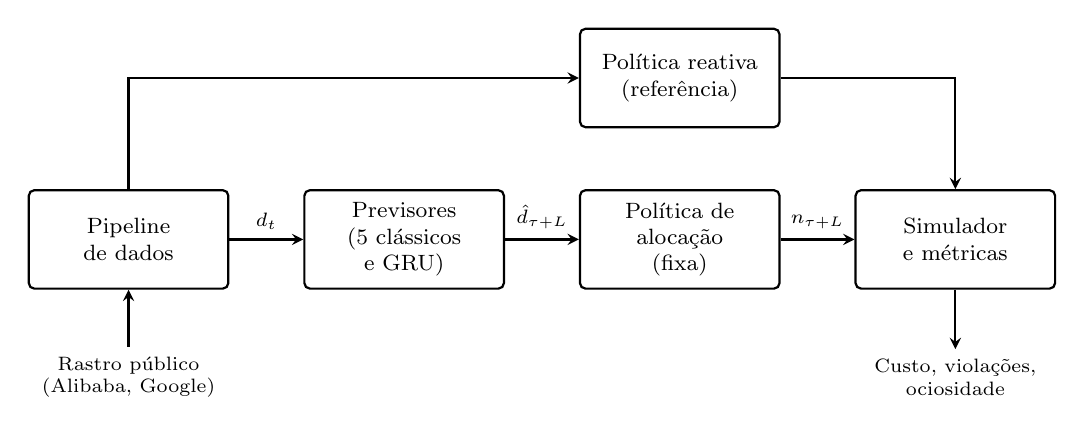
\begin{tikzpicture}[
    >=stealth, thick,
    comp/.style={draw, rounded corners=2pt, align=center, minimum height=1.25cm,
                 text width=2.3cm, font=\footnotesize},
    dado/.style={align=center, font=\scriptsize, text width=2.2cm},
]
\node[comp] (dados) at (0,0)    {Pipeline de dados};
\node[comp] (prev)  at (3.5,0)  {Previsores\\(5 clássicos e GRU)};
\node[comp] (pol)   at (7.0,0)  {Política de alocação\\(fixa)};
\node[comp] (sim)   at (10.5,0) {Simulador e métricas};
\node[dado] (raw)   at (0,-1.75)   {Rastro público\\(Alibaba, Google)};
\node[dado] (res)   at (10.5,-1.75) {Custo, violações,\\ociosidade};
\node[comp] (reat)  at (7.0,2.05) {Política reativa\\(referência)};
\draw[->] (raw)  -- (dados);
\draw[->] (dados) -- node[above, font=\scriptsize] {$d_t$} (prev);
\draw[->] (prev)  -- node[above, font=\scriptsize] {$\hat{d}_{\tau+L}$} (pol);
\draw[->] (pol)   -- node[above, font=\scriptsize] {$n_{\tau+L}$} (sim);
\draw[->] (sim)   -- (res);
\draw[->] (dados.north) |- (reat.west);
\draw[->] (reat.east) -| (sim.north);
\end{tikzpicture}
\caption{Arquitetura da solução proposta. A política de alocação é a mesma para todos os previsores; a política reativa recebe a demanda observada diretamente, sem previsão.}
\label{fig:arquitetura}
\end{figure}

\textbf{Pipeline de dados.} Converte um rastro público de \textit{cluster} em uma série de demanda com intervalos de cinco minutos, expressa em máquinas equivalentes totalmente utilizadas (utilização média de processador das $N$ máquinas, dividida por 100 e multiplicada por $N$).

\textbf{Previsores.} Cinco métodos tradicionais (ingênuo, média móvel, sazonal ingênuo, Holt-Winters e ARIMA; Seção~\ref{subsec:estatisticos}) e uma GRU univariada que, a partir das últimas seis horas, prevê todos os horizontes de uma só vez (estratégia direta; Seção~\ref{subsec:recorrentes}). Todos compartilham uma interface que só dá acesso ao histórico anterior à origem da previsão.

\textbf{Política de alocação.} Aplica uma margem de segurança $m$ sobre a demanda prevista (Equação~\ref{eq:alocacao-margem}). Como referências, há uma política reativa no estilo do \textit{Horizontal Pod Autoscaler} do Kubernetes (Equação~\ref{eq:hpa}) \cite{kubernetes2024hpa}, o dimensionamento fixo pelo pico do treino e um oráculo que conhece a demanda futura.

\textbf{Simulador e métricas.} Reproduz, intervalo a intervalo, um centro de dados com instâncias homogêneas e atraso de provisionamento, contabilizando as métricas da Seção~\ref{subsec:metricas}.

A decisão metodológica central é manter a política de alocação \textbf{fixa} e variar apenas o previsor. Assim, qualquer diferença de custo ou de violações entre duas configurações pode ser atribuída à previsão, e não à regra de decisão.

\section{Objetivos}
\label{sec:objetivos-especificos}

\subsection{Objetivo geral}

Avaliar, em um centro de dados simulado alimentado por rastros públicos de \textit{clusters} reais, a redução de custo operacional obtida pela alocação proativa guiada por uma rede neural recorrente, em comparação com métodos tradicionais de previsão submetidos à mesma política e com uma política reativa, para limites fixos de violação de SLA.

\subsection{Questões de pesquisa}
\label{subsec:questoes}

\begin{description}[leftmargin=1.2cm, style=nextline]
    \item[QP1] Para um mesmo limite de violações $\varepsilon$, a alocação guiada pela rede neural tem custo menor do que a guiada pelos métodos tradicionais? De quanto é a diferença?
    \item[QP2] Um previsor com menor erro (RMSE, MAE) leva necessariamente a uma alocação mais barata no ponto de operação?
    \item[QP3] Qual é o ganho da alocação proativa em relação à reativa, e como ele varia com o atraso de provisionamento $L$?
    \item[QP4] As conclusões obtidas no rastro da Alibaba se mantêm no rastro do Google?
\end{description}

\subsection{Objetivos específicos}

\begin{enumerate}[label=\textbf{OE\arabic*}, leftmargin=1.4cm]
    \item \textbf{Dados:} agregar o Alibaba Cluster Trace de 2018 \cite{alibaba2018trace} em série de 5 minutos, com tratamento de lacunas, divisão cronológica e relatório de qualidade.
    \item \textbf{Previsores:} implementar os seis previsores e avaliá-los por MAE, RMSE, MAPE, viés e taxa de subestimação em cada horizonte.
    \item \textbf{Simulador e políticas:} implementar o simulador e as políticas da Seção~\ref{sec:solucao} (Equação~\ref{eq:politica-preditiva}), validados por testes automatizados.
    \item \textbf{Custo e violações (QP1, QP3):} obter os pontos de operação para $\varepsilon = 1\%$ e $5\%$ (Equação~\ref{eq:calibracao}) e as curvas de custo contra violações.
    \item \textbf{Erro e custo (QP2):} confrontar o erro da previsão de horizonte $h = L$ com o custo no ponto de operação.
    \item \textbf{Sensibilidade (QP3):} medir o efeito do atraso de provisionamento $L$ sobre os pontos de operação.
    \item \textbf{Robustez:} repetir o treinamento da GRU com várias sementes e avaliar em várias janelas de teste, reportando média e dispersão.
    \item \textbf{Replicação (QP4):} aplicar o mesmo protocolo ao Google Cluster Trace de 2019 \cite{wilkes2020google}, alterando apenas a leitura dos dados.
    \item \textbf{Reprodutibilidade:} manter código e configurações em repositório público \cite{rosas2026repo}, regenerando todas as tabelas e figuras com um único comando.
\end{enumerate}

\section{Escopo do sistema}
\label{sec:escopo-sistema}

O sistema é um \textbf{ambiente de simulação e avaliação}, e não um autoescalador para produção. Recebe um rastro de utilização e um arquivo de configuração e produz tabelas e figuras com as métricas de previsão e de alocação; nenhum parâmetro é fixado no código. A Tabela~\ref{tab:parametros} resume os parâmetros do protótipo construído no Projeto Final I, que serão mantidos no Projeto Final II, salvo os ajustes decorrentes de OE6 a OE8.

\begin{table}[htbp]
\centering
\caption{Parâmetros do protocolo experimental adotados no protótipo.}
\label{tab:parametros}
\footnotesize
\begin{tabularx}{\textwidth}{>{\raggedright\arraybackslash}X >{\centering\arraybackslash}p{1.7cm} >{\raggedright\arraybackslash}p{5.6cm}}
\toprule
\textbf{Parâmetro} & \textbf{Símbolo} & \textbf{Valor} \\
\midrule
Intervalo de agregação & $\Delta$ & 5 minutos \\
Divisão cronológica (treino/validação/teste) & -- & 60\% / 20\% / 20\% \\
Horizontes de previsão avaliados & $h$ & 1, 2, 3 e 6 intervalos (5 a 30 min) \\
Janela de entrada da GRU & $w$ & 72 intervalos (6 h) \\
Período sazonal (sazonal ingênuo, Holt-Winters) & -- & 288 intervalos (1 dia) \\
Atraso de provisionamento & $L$ & 1 intervalo; 2 na análise de sensibilidade \\
Instâncias no pico do treino & $n_{\mathrm{pico}}$ & 50 \\
Custo por instância e intervalo & $c$ & 1 \\
Número mínimo de instâncias & $n_{\min}$ & 1 \\
Grade de margens (política preditiva) & $m$ & 0 a 0,60, com passo 0,01 \\
Grade de utilizações-alvo (política reativa) & $u^{*}$ & 0,50 a 0,99, com passo 0,01 \\
Tolerância e estabilização (política reativa) & -- & 10\% e 6 intervalos \\
Limites de violação & $\varepsilon$ & 1\% e 5\% \\
\bottomrule
\end{tabularx}
\end{table}

Valem as simplificações do Capítulo~\ref{cap:situacao-atual}: demanda de processador agregada, capacidade em instâncias homogêneas e violação de SLA sempre que a demanda de um intervalo excede a capacidade. A memória não restringe a alocação, pois sua utilização agregada no rastro da Alibaba varia pouco. Os itens fora do escopo são os da Seção~\ref{sec:escopo}.

\section{Usuários e situações apoiadas}
\label{sec:usuarios}

O ambiente se destina a pesquisadores e a engenheiros responsáveis pelo planejamento de capacidade que precisam decidir se a adoção de um previsor mais complexo se paga em custo de infraestrutura. Ele apoia três situações: comparar previsores sob um mesmo limite de violações antes de levá-los à produção; estimar o custo de operar com um dado nível de serviço e atraso de provisionamento; e estender a avaliação a novos previsores, políticas ou rastros, o que exige apenas implementar a interface comum do componente correspondente.

\section{Avanços em relação às soluções existentes}
\label{sec:avancos}

Os trabalhos de previsão comparam vários modelos, mas apenas por métricas de erro \cite{xu2022esdnn, rossi2023forecasting, agullo2025enhancing}, enquanto os que acoplam previsão e alocação usam um único previsor, comparado com políticas reativas \cite{calheiros2015arima, pan2023magicscaler} (Seção~\ref{sec:comparativo}). Em relação a esse cenário, o trabalho busca:

\begin{itemize}
    \item \textbf{Comparação controlada:} previsores do ingênuo à rede neural sob a mesma política, simulador e dados, combinação ausente na Tabela~\ref{tab:comparativo}.
    \item \textbf{Avaliação pelo custo a um mesmo nível de serviço:} com instâncias discretas e atraso de provisionamento, o que capta a assimetria entre superestimar e subestimar a demanda, diferentemente de \citeonline{rossi2023forecasting}.
    \item \textbf{Ligação explícita entre erro e custo:} a QP2 testa a hipótese, implícita na literatura e posta em dúvida por \citeonline{agullo2025enhancing}, de que menor erro implica melhor alocação.
\end{itemize}

\noindent Todo o experimento usa rastros públicos e código aberto, ao contrário de avaliações com dados privados \cite{pan2023magicscaler}. O trabalho não propõe uma nova arquitetura nem busca superar o estado da arte em erro de previsão: a GRU é deliberadamente simples. A contribuição está em medir o valor operacional da previsão.

\section{Itens a serem implementados e apresentados à banca}
\label{sec:entregaveis}

A Tabela~\ref{tab:entregaveis} relaciona os itens a serem entregues e sua situação ao fim do Projeto Final I. O protótipo já cobre o \textit{pipeline} completo, dos dados brutos às curvas de custo contra violações; o que foi realizado e as dificuldades encontradas são discutidos no Capítulo~\ref{cap:plano-acao}.

\begin{table}[htbp]
\centering
\caption{Itens a serem implementados e situação ao fim do Projeto Final I.}
\label{tab:entregaveis}
\footnotesize
\begin{tabularx}{\textwidth}{>{\raggedright\arraybackslash}X >{\centering\arraybackslash}p{1.6cm} >{\raggedright\arraybackslash}p{5.2cm}}
\toprule
\textbf{Item} & \textbf{Objetivo} & \textbf{Situação no PF~I} \\
\midrule
\textit{Pipeline} de dados & OE1 & Implementado \\
Previsores & OE2 & Implementado \\
Simulador e políticas & OE3 & Implementado \\
Experimentos de custo, violações e erro contra custo & OE4, OE5 & Preliminar (uma semente, uma janela de teste) \\
Análise de sensibilidade & OE6 & Parcial ($L = 1$ e $L = 2$) \\
Avaliação robusta & OE7 & Previsto para o PF II \\
Replicação no Google & OE8 & Previsto para o PF II \\
Repositório reprodutível & OE9 & Implementado; a ser mantido \\
Relatório final e apresentação & -- & Previsto para o PF II \\
\bottomrule
\end{tabularx}
\end{table}

Na defesa, serão apresentados: (i) as curvas de custo contra violações e os pontos de operação de todos os previsores e da política reativa, nos dois rastros; (ii) a comparação entre a ordenação dos previsores por erro e por custo; (iii) a análise de sensibilidade ao atraso de provisionamento; e (iv) a regeneração dos resultados a partir dos dados brutos pelo repositório.

Duas extensões, condicionadas ao cronograma e fora do compromisso de entrega, podem ser avaliadas no mesmo arcabouço: a previsão multivariada com memória como entrada adicional, nos moldes do esDNN \cite{xu2022esdnn}, e a substituição da margem fixa por um quantil previsto pela rede \cite{rossi2023forecasting, pan2023magicscaler}.